\documentclass[12pt,a4paper]{article}
\usepackage{graphicx}
\usepackage{hyperref}
\graphicspath{ {E:\301\Coding\Standards/ } }

\hypersetup{      
    urlcolor=blue,
}
\urlstyle{same}


\begin{document}
	\begin{titlepage}
		\begin{figure}[t]
			
\includegraphics[scale=0.5, height=2cm, width=10cm]{ThutongLogo.png}
		\end{figure}
		\centering
		
		\textbf{\LARGE Digital BlackSmiths: Thutong LMS}
		\newline
		\rule{\textwidth}{1.6pt}\\[\baselineskip]
		\textbf{\Large Coding Standards Document}\\
		\vspace*{0.5cm}
		\large{Group Members:}\vspace*{0.3cm}
		\\{Fiwa Lekhulani\\Daniel Rocha\\Lebogang Ntatleng\\Lesego Mabe\\Tlou Lebelo}
		\rule{\textwidth}{1.6pt}\\[\baselineskip]
		
		
		\vspace*{\fill}
	\end{titlepage}


	\date{\textbf{\today}}
	\pagenumbering{roman}
	%\noindent\rule{\textwidth}{1pt}
	\pagebreak
	\tableofcontents
	\newpage
	\pagenumbering{arabic}


	This document contains the coding conventions created by the Digital Blacksmiths team, based on the various languages used to create the Thutong Online Learning System.
	\newline
	The team makes use of Moodle, JavaScript and *** for the creation of the system.\\
	Moodle is purely coded in PHP and coding standards are defined at \url{https://docs.moodle.org/dev/Coding_style} \\
	The rest of this documentation will describe the coding conventions used for the remainder of the languages used.	
	
	\section*{Detailed System Design}
	%UML
	\begin{figure}[h]
			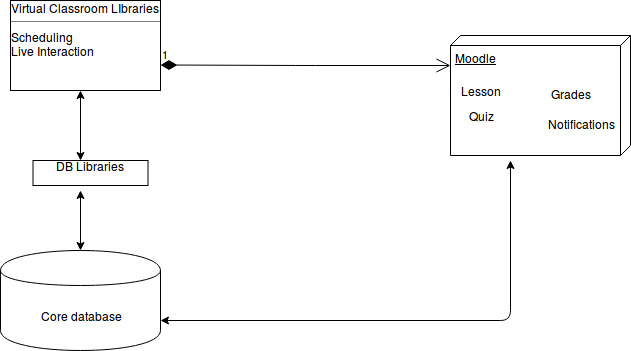
\includegraphics[width=10cm]{System.jpg}
		\end{figure}
		%decription of system
	
	\section*{Coding Conventions}
	To ensure that the code is flexible, readable, reliable and efficent the following aspects are considered and given the stipulated rules:	
	
	\subsection*{Naming Conventions}
		\begin{itemize}
			\item Classes, functions and variables are to be named to descriptive as to what their purpose is.
			\item e.g
		\end{itemize}		
	
	\subsection*{Layout Rules}
	The structure of each file must adhere to the following  layout:
		\begin{itemize}
			\item Each file must have a file header wherein which the location, version, author and update history\newline When a change is made to the file, the developer is required to change the date for last updated
			\item Only one class is allowed within a file, which may have infinite internal functions
			\item A class must have a description for its overall functionality and it's internal functions
			\item No more than one blank line is prohibited between lines of code, but with that said functions must be separated with a blank line for clarity and readability
			\item Every class definition, function and loop must be indented. The beginning brace must be placed in the same line as the definition of the loop or function but the ending brace must be in its own line followed an empty line.
			\item Code must be neat and self-explanatory, comments should be used when an action is fairly
complex or needs additional instruction to another programmer.
		\end{itemize}
		
	\subsection*{Commenting Practices}
		\begin{itemize}
			\item File header are composed of multi-line comments
			%e.g. image
			\item class or function definitions are made preceding the function using single line comments; these comments must be brief and solely give the core purpose of the class or function.
			\item Single line comments are to be used to give an explanation of what a specific line does; these should be only used when necessary. Avoid redundant commenting that can be easily understood from code naming conventions, methods and functionality.
		\end{itemize}
		
		
	\section*{File Structure}
	%git
	
	\section*{Code Review Process}
	%how and why
	Each members' code uploaded to GitHub is reviewed **(after it is committed/weekly/monthly)*** to ensure that it complies with all above-mentioned standards and so that all group members understand the purpose of newly uploaded code for overall understanding of the system and newly added functionality. 
	
	
\end{document}